\definecolor{darkgreen}{rgb}{0.0, 0.5, 0.13}
\definecolor{darkred}{rgb}{0.55, 0.0, 0.0}
\newcommand{\gct}{\color{darkgreen}\checkmark}
\newcommand{\rma}{\color{red}\ding{55}}
\newcommand{\bct}{\color{blue}\checkmark}

\newcommand{\arrowdownunder}{\begin{center}$\big\downarrow$\end{center}\vspace{-0.3cm}}
\newcommand{\mycolutitle}[1]{\vspace{-0.7cm}\begin{center}#1\end{center}\vspace{-0.1cm}}

\author[Juan Cruz-Martinez]{}
\institute{University of Milan}

\subsection{A new generation}
\begin{frame}[t]
    \frametitle{Key differences with respect to the 3.1 methodology}
    \footnotesize
    \begin{columns}[t]
        \column{0.5\linewidth}
            \mycolutitle{NNPDF 3.1 code}
            \begin{list}{\color{darkred} $\rightarrow$}{}  
                \item {\bf Genetic Algorithm optimizer}
                \item One network per flavour
                \item Physical constraints imposed independently of optimization
                \item Preprocessing fixed per each of the replicas
                \item C++ monolithic codebase
                \item In-house Machine Learning optimization framework
                \item Fitting times of up to various days
            \end{list}
            \arrowdownunder
            \begin{itemize}
                \item[]{\bf Fit parameters manually chosen \\ (manual optimization of hyperparameters)}
            \end{itemize}
        \column{0.5\linewidth}
            \mycolutitle{NNPDF 4.0 code}
            \begin{list}{\color{darkgreen} $\rightarrow$}{}  
                \item {\bf Gradient Descent optimization}
                \item One network for all flavours
                \item Physical constraints integrated in the optimization
                \item Preprocessing can be fitted within replicas
                \item Python object oriented codebase
                \item Freedom to use external libraries (default: TensorFlow)
                \item Results available in less than an hour
            \end{list}
            \arrowdownunder
            \begin{itemize}
                \item[]{\bf Fit parameters chosen automatically (hyperparameter scan)}
            \end{itemize}
    \end{columns}
\end{frame}

\subsection{Hyperoptimization and K-folding}

\begin{frame}{Beyond the PDF fit: fitting the methodology}

    The main objective of NNPDF is to minimize choices that can bias the PDF:

    \begin{columns}
        \column{0.7\linewidth}
        \begin{itemize}
            \item[\rma] Functional form $\longrightarrow$ Neural Networks
            \item[\rma] However: NN are defined by set of parameters!
        \end{itemize}

        \vspace{0.2cm}

        Humans are good at recognising patterns but selecting the best
        set of parameters is a slow process and systematic success is not guaranteed
        \column{0.2\linewidth}
        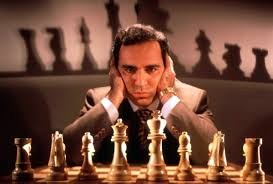
\includegraphics[width=\textwidth]{juan_future_hyperopt/kasparov.jpg}

        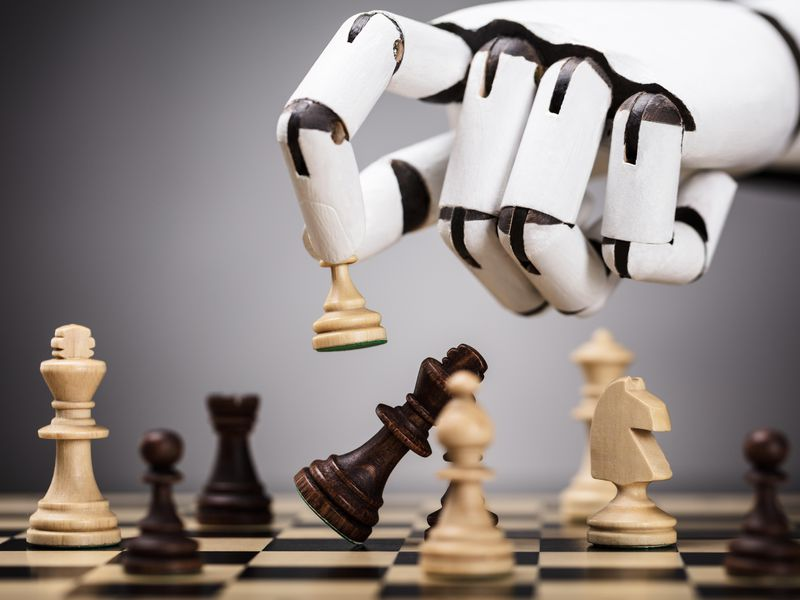
\includegraphics[width=\textwidth]{juan_future_hyperopt/alphazero.jpg}
        \column{0.1\linewidth}
    \end{columns}

    \vspace{0.2cm}

    To overcome this selection problem we implement a {\color{blue}  hyperparameter scan}: let the computer decide automatically

    \begin{itemize}
        \item[\gct] Scan over thousands of hyperparameter combinations
        \item[\gct] Define a reward function to grade the model
        \item[\gct] Check the generalization power of the model
    \end{itemize}

\end{frame}

\begin{frame}
    \frametitle{Hyperparameter scan} 
    Each blue dot corresponds to a fit of a different set of hyperparameters:
    { 
        \centering 

        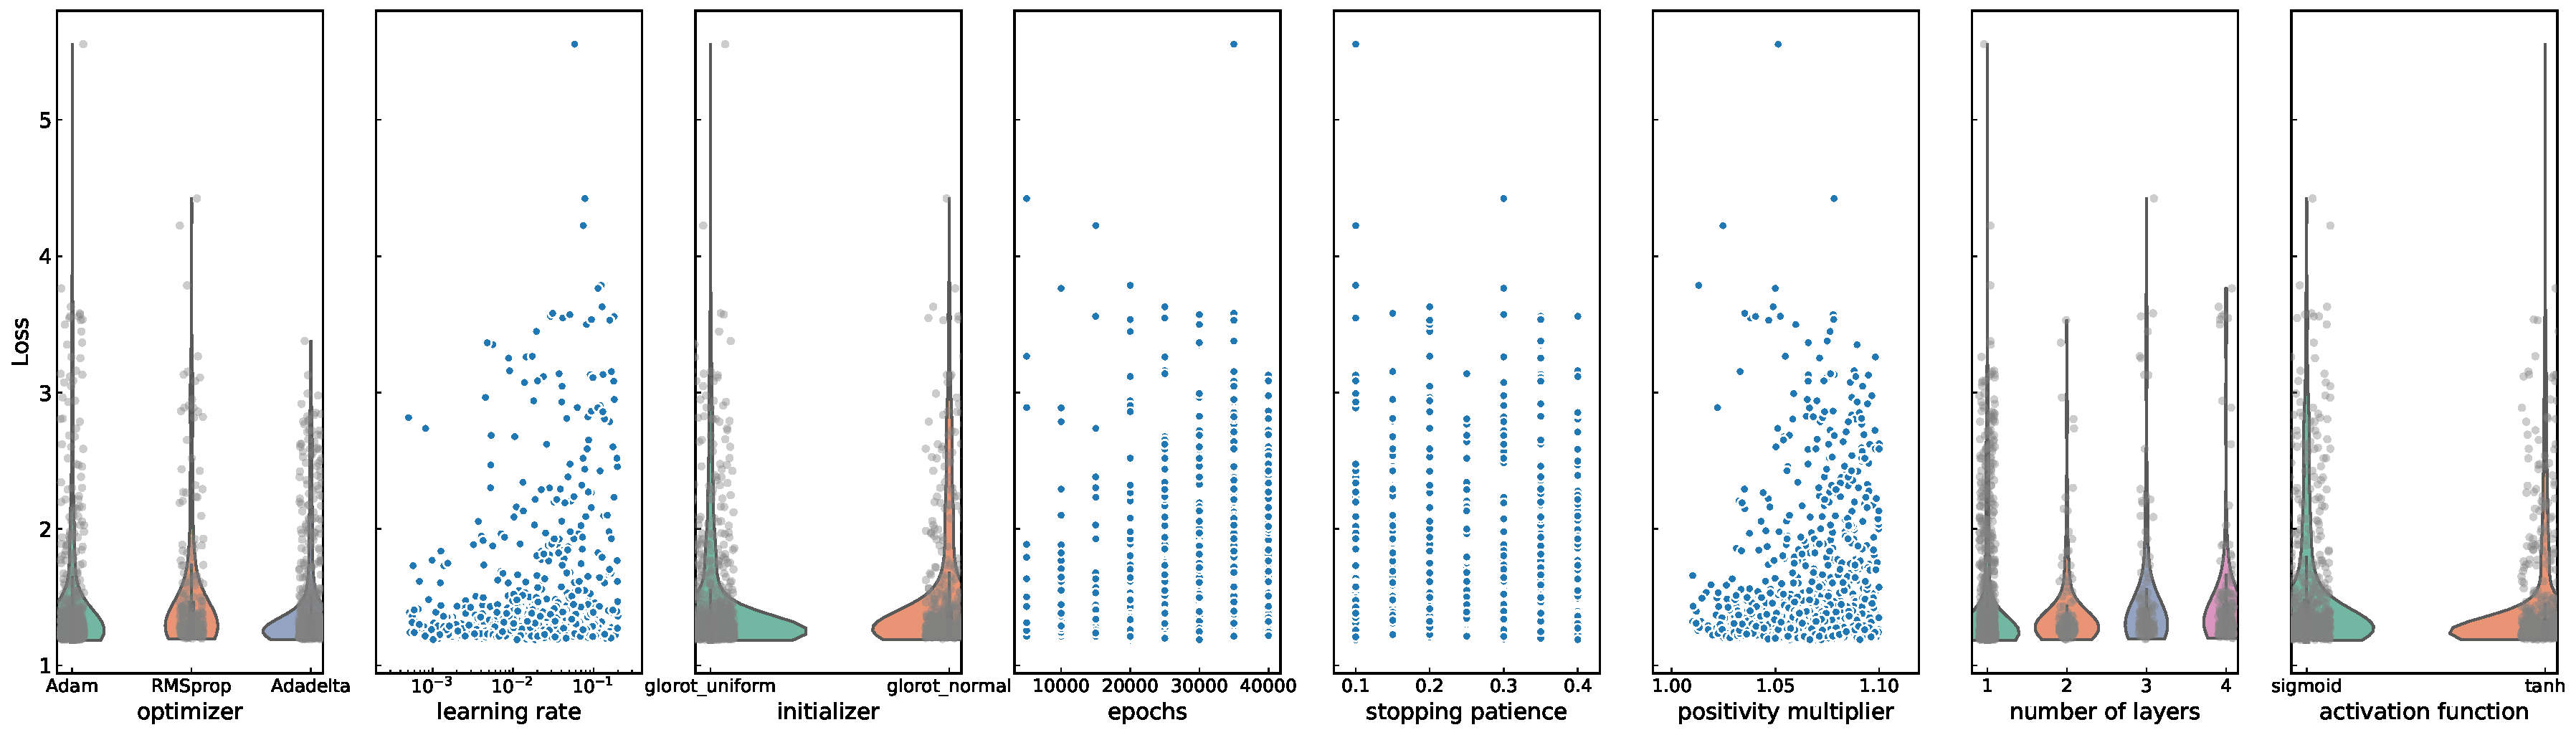
\includegraphics[width=\textwidth]{juan_future_hyperopt/dis-fullpage.pdf}
        Thousands of fits for the hyperoptimization algorithm to choose:

        \begin{columns} \small
            \column{0.35\paperwidth}
            \begin{itemize}
                \item[\bct] Optimizer
                \item[\bct] Initializer
                \item[\bct] Stopping Patience
                \item[\bct] Number of Layers
            \end{itemize}
            \column{0.35\paperwidth}
            \begin{itemize}
                \item[\bct] Learning Rate
                \item[\bct] Epochs
                \item[\bct] Positivity Multiplier
                \item[\bct] Activation Function
            \end{itemize}
        \end{columns}
    } \vfill
\end{frame}

\begin{frame}
    \frametitle{Hyperoptimization: reward and generalization}
    If we use as hyperoptimization target the $\chi^{2}$ of the fitted data, we risk finding the hyperparameter set that
    better overfits.


    \vfill

    \begin{columns}
        \column{0.75\linewidth}
        We avoid this problem by adopting \textbf{$\boldsymbol{k}$-folding}:

        \begin{itemize}
            \item Divide the data into $k$ sets.
            \item Leave one set out and fit the $k-1$ sets left.
            \item Optimize the average $\chi^{2}$ of the $k$ non-fitted sets.
        \end{itemize}
        \column{0.25\linewidth}
        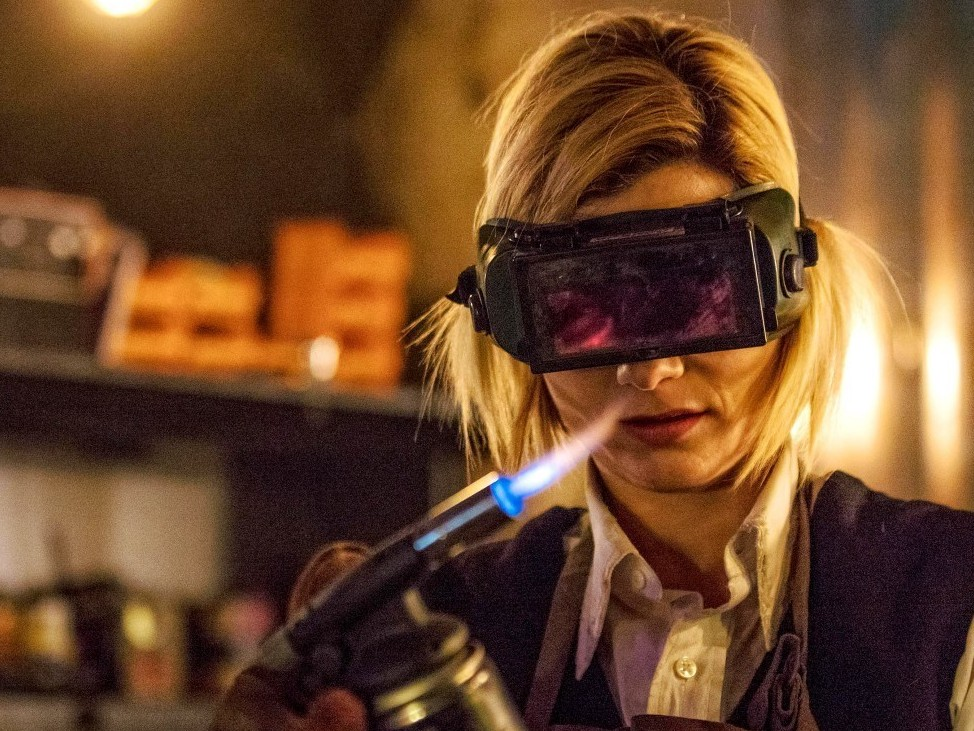
\includegraphics[width=\textwidth]{juan_future_hyperopt/doctor.jpg}
    \end{columns}

    \vspace{0.4cm}

    Example of function to hyperoptimize:

    \begin{equation*}
        \text{Loss}(optimizer\_name,\ depth\_of\_network) = \frac{1}{k}\displaystyle\sum^{i}_{k} \frac{\chi^{2}_{i}}{N_{i}}
    \end{equation*}

    Where we are computing the $\chi^{2}$ for the data that did not enter the fit. This ensures that the methodology
    can accommodate well even data that has never been seen by the fit.

\end{frame}
